\chapter{Motivation}

This guideline for composing master theses, seminar papers and lab reports was
inspired by the observation that, in the process of their work, students often
repeat the same mistakes that could easily be avoided. On this background, the
idea for this guideline was born with the intention to reduce your (and also,
of course, our) time input, and provide you with a set of techniques for composing
scientific texts which have proven very effective for improving the presentation of
contents as well as as their comprehensibility for the reader.


\section{The Purpose of a Lab Report}

Preparing the report is an inherent part of every lab offered by our work group
during the main study period. The report should give the reader a detailed picture of
 
\begin{itemize}
\item which task was tackled during the practical exercises,
\item which challenges had to be coped with in order to accomplish the task,
\item in what way and how well these challenges were mastered.
\end{itemize}

The report is \textbf{not a protocol of procedures}, i.e. it should not provide a
detailed listing of all steps made in order to solve the problem. It is rather a
documentation of the applied solution and should also motivate why this particular
solution was chosen. It can be appropriate to also mention other possible solutions
that were tried but lateron abandoned for good reasons. However, the description of
the implemented solution must definitely outweigh such references.


\section{The Purpose of a Seminar Paper}

A seminar paper should summarize in short the vital aspects of a given subject.
Since the size of the text sources usually outnumbers the admitted paper volume by
far, it is inevitable for the author to reduce the sources to the relevant facts.
The paper should be written in the author's own words and never be literally copied
from the original text. This rule particularly applies to text sources in foreign
languages: literal translations are usually easy to recognize for the simple reason
that they are difficult to read; apart from that, they simply miss the point of the
matter. One of the excuses for using literal translations is that the original text
could not be understood. If this is the case, rather consult your tutor for help --
that is what he is there for. Other popular excuses like "This source was so
excellent, I could not have said it better" certainly do not require any further comments.


\section{The Purpose of a Master Thesis}
\label{sec:aufgaben-diplom}

According to the MaPO (conditions of study) of 2011 \cite{mpo11}, the Master thesis is defined as (original quotation from the German language MaPO):

\begin{bigquote}{\cite{mpo11}}
  "\S 17 (1) Die Masterarbeit ist eine schriftliche Prüfungsarbeit, die zeigen soll, dass der Prüfling in der Lage ist, innerhalb einer vorgegebenen Frist ein Problem aus dem Gebiet des Studiengangs selbständig nach wissenschaftlichen Methoden zu bearbeiten, einer Lösung zuzuführen und diese angemessen darzustellen. [...] Die Masterarbeit soll auf Englisch verfasst werden. 
\end{bigquote}

A corresponding English meaning would be:
\begin{bigquote}
 ... the master thesis is expected to show that the student is capable of 
  independently applying scientific methods to a problem in the field of computer science within a set period of time,
  proving his/her aptitude for self-dependent scientific work. [...] The master thesis should be written in english.
\end{bigquote}

The Master thesis is reviewed on the basis of the written elaboration handed in by
the student. Therefore, for the student's own benefit it is recommended to focus not
only on the contents, but also on an appealing form of their presentation. Normally,
the grade is not strongly influenced by formal aspects of the thesis. If, however,
we have to make a choice between two possible gradings, the form of presentation can
be of vital significance.


\chapter{Choosing the Appropriate Tool}

Prior to starting the actual writing process, the student has to decide which text
processing program he will use. The answer to this question is quite easy to give:
Basically we do not have any preference as to the tools used as long as we receive
the result as a \textbf{PDF-file}.


\section{LaTeX}

LaTeX (spoken:"Lahtech") (\cite{latex_book,latex}) sets scientific texts
in premium quality. Comparing LaTeX with other text processing programs, like MS Word
or Open Office, you will easily note the difference in quality. Also, LaTeX is highly
reliable; it will not fail even with the 100th page, the 100th reference, the 100th
mathematical formula and the 100th picture within one document.

Those who have so far worked only with WYSIWYG-tools might have to get used to
giving layout instructions by embedding the respective LaTeX commands in the text.
Also, some (few) basic structures have to be understood. Once the necessary
"working set" of LaTeX-structures is established, the composition of
further texts with LaTeX will be very easy.

On this background, it is recommended that you get used to working with LaTeX as early
as possible, for example in the course of working on the seminar paper or lab report.
A lot of excellent assistance can be found in the Web, for example on the site of
DANTE e.V. (\cite{dante}).


\section{Open Office, MS Word, etc.}

From a very simplified point of view, there are as many shortcomings to LaTeX as there
are advantages to common WYSIWYG text processing programs, such as Open Office or MS Word
(and vice versa), where it is possible to start working right away and quickly get to
an acceptably formatted result. The difficulties often start in the course of working
on long texts containing numerous pictures and formulas, since they will lead to a rapid
decrease of reliability and processing speed.


\section{Recommendation}
Basically, our experience shows that LaTeX is the best choice when working with complex
documents. The initial work input which is necessary to get used to this tool will lateron
be rewarded by high stability, a minimum of layout work, high print quality, and, last
but not least, a significant reduction of trouble.


\chapter{Structure}

A very common method of starting an elaboration is the so-called \emph{top-down},
i. e. the drafting of an appropriate structure of chapters that lateron will
be refined and filled with text. The most basic structure divides the text
into introduction, main part, and conclusion.
 

\section{The Introduction}

Ideally, the introduction convinces the reader that it is worthwhile reading the
rest of the paper, i.e. it should name the tasks of the work and explain
why their investigation is of interest. In order to demonstrate the relevance
of a problem it can be helpful to present it in a larger context.

While the beginning of the introduction should sufficiently motivate the reader 
to continue reading, the end of the introduction should give a survey of the
chapters to follow, outlining in short how the task was approached.


\section{The Main Part}

The main part is the actual core of the paper and consists of several chapters
which in terms of argument and presentation should form a logical line.
Lab reports and Master theses often require the following structure, with each
point possibly leading to several chapters:


\begin{description}
  
\item[Introduction of basics] First of all, it is important to
  introduce the basic concepts of the work. It can be taken for granted
  that the reader is familiar with the contents of the lecture 
  "High Performance Networking (MA-INF 3101)" (for seminar or lab in the
  second semester) and of the lecture(s) "Network Security (MA-INF 3201)"
  and/or "Mobile Communication (MA-INF 3202)" (for seminar, lab or 
  Master thesis in the third or higher semester). By no
  means we must lapse into writing a piece of universal technical literature.
  It is important to introduce only those basics that the paper/thesis will
  lateron refer to. Additional details of no relevance for the work will just
  distract the reader's attention and not only waste space but also
  strain the reader's (and the assessor's :-)) patience.
  
\item[Specification of the task] Whereas in the introduction the task 
  was outlined rather abstractly and in a larger context, it should now be
  specified: What exactly will be examined in this work (and what will not)?
  
\item[Description of possible solutions] Drawing upon the former
  chapters, we now have to develop our own solutions. To "look beyond
  one's own nose" and document what others hitherto contributed to the
  task are essential parts of scientific work. If task-related works do exist,
  it is good to emphasize the differences between them and our own work.

\item[Assessing the methods of solution] It is easy to allege things!
  However, it needs formal evidence or an empirical proof to make a statement
  valuable. Therefore, a significant part of the work accounts for examining the
  methods of resolution. This is the place for presenting analytical, simulative,
  or prototypical measuring results in order to emphasize the quality and special
  applicability of our own method (in comparison with other approaches). The
  "road" leading from assumptions to conclusions should be comprehensible
  for the reader to an extent that enables him to repeat the research for 
  verification.

\end{description}

If the length of a chapter exceeds a certain limit, it is helpful to start with a
brief introduction that picks up the thread leading through the document and outlines
the contents of the following chapter. Also, each chapter should end with a short
summary stressing essential points of the chapter.


\section{The Conclusion}

The final chapter ("Summary") summarizes the primary aspects of the work
and present its essence. The summary should be comprehensible even for readers who
are not familiar with the contents of the main part. The reader, just by reading the
introduction and the summary, should get an idea of the document's tasks as well as
their solutions.

Also, this is the adequate place for presenting our own notions about the task in a 
short résumé.

In lab reports and Master theses, conclusion should also mention the prospects
of possible further work, especially questions that arose in the course of the
work but for reasons of time and/or space could not be dealt with in depth.

\section{The Volume of a Paper}
The volume of a paper consists of the amount of pages beginning with \emph{the first page of the introduction} and ending with the \emph{last page of the summary}. Hence, the cover page, the table of contents, reference lists, and attachments do \emph{not} count as parts of the volume. Only the plain plain text will be counted. Here are some tried and tested benchmarks for the volume of different kinds of papers and scripts:

\begin{itemize}
\item 25--100 pages for a Master thesis (see \cite{mpo11} \S 17 (5)),
\item 5--10 pages for a seminar paper (see \cite{mpo11} \S 16 (3)),
\item 15--20 pages for a lab report.
\end{itemize}

If the paper/report/thesis exceeds the given volume, it should be reconsidered whether the conceptual formulation is too complex and, with the tutor's agreement, needs to be reduced.

\chapter{The Correct Usage of ...}
... \emph{heading}. Well \textbf{two headings should never follow each other directly}. The reader does not understand why you separated the following chapters from each other. Explain it to them. In this case we discuss the correct usage of a multitude of different concepts. Within the following sections we introduce them in depth.

\section{Footnotes}
Footnotes were invented by the humanities, where dealing with research sources is of high significance. Footnotes here mainly serve as references to the source of a citation. In the field of computer science, however, footnotes are \textbf{used rather scarcely}. If a reference to an external source is required, the source will be referenced (see chapter \ref{sec:references}).

Footnotes are often used for remarks that are not supposed to appear within the  actual text. However, if the remark is important enough to be mentioned, it can as well be placed in the main text. Otherwise it is probably not that important and we can deal without it.  \footnote{Do you realize how this meaningless footnote obstructs the read flow?}


\section{Page Numbers}
Page numbers are important for the simple reason that the printed document is not always stapled when it lies on a desk, and a draft through the open door is sometimes enough to sweep the whole stack off the desk and turn it upside down.
In addition, page numbers are very helpful in the process of reviewing ("The first paragraph on page 67 should be rephrased"). Therefore, we recommend to \textbf{always use page numbers}. If you use the template you \emph{will} have page numbers.


\section{Figures}
\label{sec:figures}
Figures are meant to improve the comprehensibility of the text and should therefore be \textbf{generously applied} (mind that "generously" must not be taken too literal). According to our experience, an average of one figure in \textbf{2-3 pages} is acceptable. Too many figures would cause the impression of a comic strip.

A figure says more than a thousand words, however, it can not replace descriptive comments in the text. A general rule says that a figure should support the comprehension of a text, but by no means can be planted into it without further explanation. It is important to always make sure that the text provides \textbf{references and descriptions} to the figures. In addition, each figure should be captioned in an explanatory way.


    \begin{example}
      \subsubsection*{Example:}
      TCP and IP have different functions. Figure \ref{fig:1} shows the
      interaction of both protocols during the communication of the two
      nodes A and B that are interconnected via several routers. IP, being
      the protocol analog to the third layer in the OSI-Model, has the
      function of ... \emph{(... continue discussion of the figure)}
     \end{example}

  \begin{figure}[ht]
    \begin{center}
      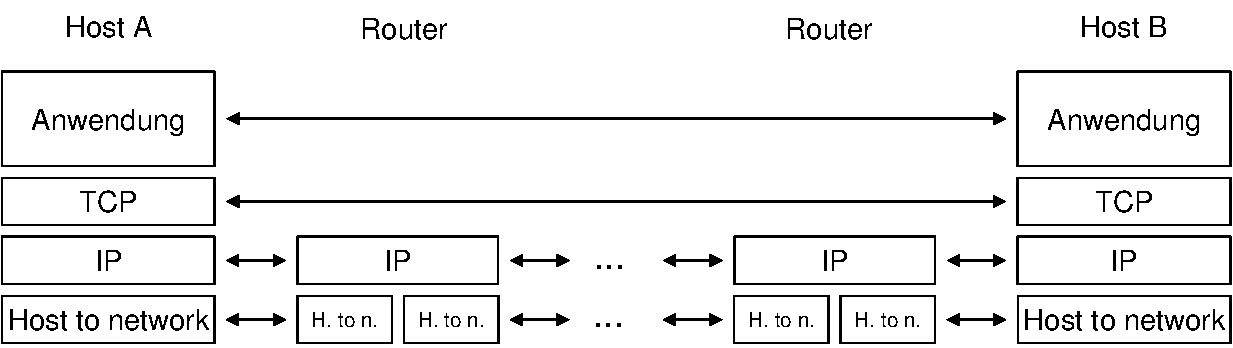
\includegraphics[width=\textwidth]{fig/communication}
      \caption{The TCP/IP protocol stack during the communication process
        between two hosts}
      \label{fig:1}
    \end{center}
  \end{figure}



\subsection{Figures of Other Authors}
Lots of figures have been created, among them may even be figures that
exactly match your work. If you find such a figure, you might want to use
it in your paper/thesis. In this case you have to make a \textbf{figure reference} to the source of the figure; either in the figure itself or in the annex.

If you wish to use a figure that is not available in an electronic format,
the simplest of all solutions is to scan it. If the figure is part of an
electronic document, you can make a screenshot. Mind that, using this type
of figures, it is important to choose a sufficiently high resolution to ensure that the printer will not turn it into a load of "pixel mud".
At the same time, the resolution should be as low as possible in order to not
unnecessarily blow up the size of the document.

Therefore, it is worth considering to draw the picture yourself with a tool
of your own preference and embed it as a \textbf{vector graphics}.
In most of the cases you will end up having to apply changes to a foreign figure, because it eventually turns out to not 100\% match with the situation in your work.
If after that the figure still strongly resembles the source, and if it is not a commonly well-known picture, as e.g. the TCP/IP protocol stack, the source must be marked as "according to [reference]". We recommend to choose
a vector format (.wmf, .emf, .eps, .pdf), since they do not occupy much space
and scale arbitrarily without looking "pixelish".


\subsection{Colors}
A colored figure is a nice thing - provided you will use a color printer. In a black-and-white-print the colors will be reduced to their grades of brightness, as a result of which the contrast distribution will not remotely reach the intended quality. Therefore, when creating colored figures, make sure that even in a black-and-white print the necessary information will still be distinct. You can as well abstain from colors and use different shades of gray instead. In plots, different curves can be distinguished by using different line types.

However, if you wish to use colored figures, do not refer to the colors in the text. Phrases like "Active nodes are marked red, passive nodes blue and inactive nodes green" in a black-and-white print have a rather comical effect and will lead to confusion rather than comprehension.


\subsection{Plots}
Plots should be created e.g. with Gnuplot \cite{gnuplot_homepage}, R \cite{r_homepage}, OpenOffice \cite{oo_homepage}, or Excel. They can easily be embedded as vector formats, so it is not necessary to use screen shots. When using plots, it is important to \textbf{label all the axes} and indicate the \textbf{units}.

Make sure to use an \textbf{appropriate scaling}. For example, instead of saying "10000000 bps" or "1.0e-07 bps" the more concise "10 Mbps" is preferable.

An example of how not to do it is shown in figure \ref{fig:plots} (a): a pixelish Gnuplot-screenshot without units at the axes and a badly chosen scaling. Example (b) shows the same plot with a reasonable labeling as .eps import.

\begin{figure}[ht]
    \centering
    \subfigure[Poor] {
        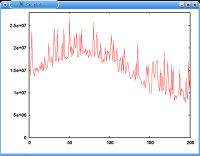
\includegraphics[width=9cm]{fig/plot_falsch_small}
    }
    \subfigure[Better] {
        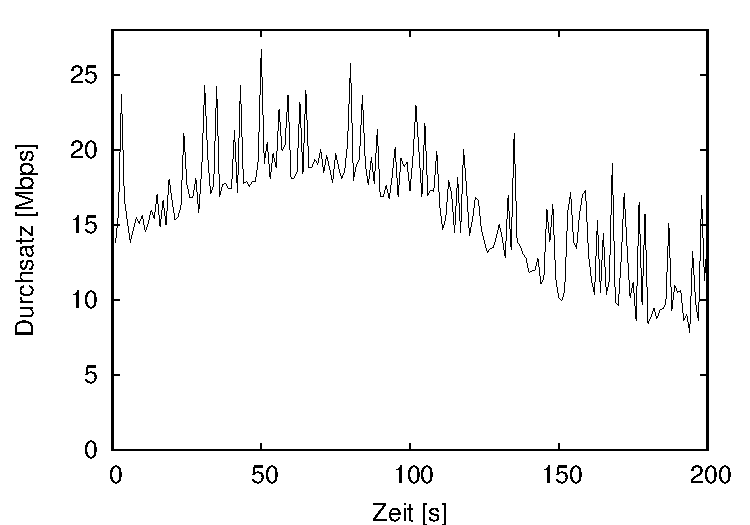
\includegraphics[width=9cm]{fig/plot_richtig}
    }
    \caption{\label{fig:plots}Examples for a presentation of measurement results}
\end{figure}


\section{Tables}
Most of the rules that apply to figures also apply for tables:
Tables have to be numbered, captioned, and referenced in the text.
The difference between tables and figures is that the caption is above the table but below a figure.
In case you wish to present extensive measurement- or simulation results, a graphic
representation could possibly convey the information more concisely than a table.

  \begin{example}
    \subsubsection*{Example:}
    To analyse the aspect XYZ, three test series were carried out
    in the test systems. Table \ref{tab:config} summarizes the
    sender- and receiver configurations used in the test series.
  \end{example}

\begin{table}
  \renewcommand{\arraystretch}{1.5} 
  \begin{center}
    \caption{Sender- and recipient configurations of the implemented test series}
    \begin{tabular}{|c|c|c|}
      \hline
      \textbf{Test Series} & \textbf{Sender} & \textbf{Recipient} \\
      \hline
      1 & heineken & grolsch \\
      \hline
      2 & heineken & bitburger  \\
      \hline
      3 & grolsch & bitburger \\
      \hline
    \end{tabular}
    \label{tab:config}
  \end{center}
\end{table}


\section{Code}
\label{sec:code}
It is often advisable to put complex algorithmic procedures in code.
These shall be noted in \emph{Pseudocode} in natural language form.
In regard to typeset the rules for figures (refer to section \ref{sec:figures}) apply to code, as well.
A small example is given in Figure \ref{code:science}, below.

\begin{algorithm}
  \KwData{Your thesis task}
  \KwResult{A thesis}

  \While{not\_finished(thesis)}{
    work\_on(thesis)\;
  }
  proofread(thesis)\;
  turn\_in(thesis)\;

  \caption{Pseudocode for compilation of a research thesis.}
  \label{code:science}
\end{algorithm}

This template includes the package \texttt{algorithm2e} \cite{pkg:algorithm2e}.
It is configured to the requirements outlined.

\section{Quotations}
\label{sec:quotations}
We recommend to not extensively quote text sources. Computer scientists usually make it short; instead of quoting a source, they reference it in the appropriate place. However, it can be helpful to now and then quote a particular paragraph containing information which is crucial for your work. In this case, the quotation has to be put in \textbf{quotation marks} and stand out against the rest of the text (for example, by indented paragraphs or italicized font). Furthermore, the source has to be indicated by a reference (see quote from the MPO in Chapter
\ref{sec:aufgaben-diplom}).

By no means quotations may be used to describe the basics of your work. Although it is easy to find elaborate introductions to most subjects, it would by far miss the purpose of your work to simply adopt them. On the contrary, they can be rather incongruous since they most probably will not confine themselves to the essentials of this aspect of your work.

If, in addition, the reference to the quotation is missing, it means that the author tries to pass off a foreign work as his own. This is called plagiarism and is incompatible with the methods of academic work which, as a purpose of our lectures, we want the students to acquire.

\textbf{If we identify a case of plagiarism, we will get very angry -
   sometimes angry to an extent that we will refuse the certificate, or grade the Master thesis as not passed.}


\section{References}
\label{sec:references}
The following chapter addresses various aspects of referencing.

\subsection{What do I reference?}
When choosing a source, it is of great importance to check its reliability.
Usually, the  books, articles of scientific magazines or conference proceedings, standards, and other sources that we make available for you undergo a scientific review to ensure a certain reliability.

Computer magazines, such as c't, iX etc., belong to a scientific twilight
zone. They do get reviewed, however, the reviews are editorial, not
scientific, hence they should be referenced for non-technical aspects only.
For example, you should \emph{not} reference a TCP/IP-tutorial from the c't or,
even worse, the Computer-Bild - more appropriate here would be a reference to books
or the relevant standards. However, in an introduction it is not at all out of
place to quote from an article about the commercial predominance of a new radio
communication standard and reference the sales figures for end devices mentioned
in the article.

You will need a good deal of skepticism when dealing with internet publications (including, among others, seminar/study papers from other authors) that were not obviously subject to review. You better avoid this kind of sources, since the internet makes it quite easy to publish the most amazing nonsense.


\subsection{How do I reference?}
Two different ways of referencing have been established. The first one are
found mainly in English publications: The references are simply bracketed and
serially numbered:

    \begin{example}
      \subsubsection*{Example:}
      An alternative mechanism for congestion
      control which recognizes congestion by the increase of round
      trip time was already introduced [1].
    \end{example}

Alternatively, the signature of the reference consists of the initials
of the authors' last names and the last 2 digits of the year of publication.
This form of referencing is most customary in German publications:

    \begin{example}
      \subsubsection*{Example:}
      An alternative mechanism for congestion
      control which recognizes congestion by the increase of round
      trip time was already intrudeced [JWL04].
    \end{example}

The following rules have proven useful for both notations:
\begin{itemize}
\item To prevent a signature from getting too long, only the first
  three authors will be mentioned. If there are more than three authors,
  this is indicated by a "+" behind the list of authors
  (e.g. [IML+01] for a paper published by Inamure, Montenegro, Ludwig,
  Gurtov, and Khafizov in 2001).

\item In case there is only one author, the first three letters of his
  last name will be indicated (e.g. [Hus01] for an article published by
  Geoff Huston in 2001).

\item If an author or a group of authors produced more than one publication
  in one year, the referenced publications of the same year will be distinguished by an attached lowercase letter (e.g. [Pos81a], [Pos81b] or [Pos81a,Pos81b]).

\item If there is no designated author or publisher (which can happen in case
  of standards), arbitrarily choose an explicit letter combination (e.g.[IEEE99] for an IEEE standard).
\end{itemize}

When it comes to the point of where to set the reference specifically, please note that the reader would like to read a sentence of words he knows.
The best choice is to phrase sentences that may be read without the reference itself. Please consider the following examples:

    \begin{example}
      \subsubsection*{Example (poor):}
      In [JWL04] we introduce an alternative mechanism for congestion
      control which recognizes congestion by the increase of round
      trip time.

      \subsubsection*{Example (better):}
      An alternative mechanism for congestion
      control which recognizes congestion by the increase of round
      trip time was already intrudeced [JWL04].
    \end{example}

Further the specific place a reference is set does matter. The validity of the reference is limited to the next punctuation mark. If a reference is used before a full stop it is valid for this sentence. If it occurs behind a full stop, but right before the end of a paragraph. It is valid for the full paragraph.

The references will be listed in a separate chapter at the end of the document. Each reference appears as a separate entry in the following format:

\begin{example}
  \begin{tabbing}
    [Signature] \= author(s), title of publication, specification about magazine,
    conference, \\ \> book in which the source was published, page number (if possible),\\
    \> year of publication, ISBN.
  \end{tabbing}
\end{example}

The information contained in the reference list has to be exhaustive enough to enable the reader to find the source (in fact, without using Google or Citeseer).


\subsubsection*{Examples for RFCs/Standards:}
\begin{example}
\begin{tabbing}
  {}[IEEE99] \= \kill \\
  {}[Pos81a] \> J. Postel, \emph{Internet Protocol}, September 1981, IETF, RFC
  791, Status: \\*
  \> Standard.\\
  {}[Pos81b] \> J. Postel, \emph{Transmission Control Protocol}, September
  1981, IETF, RFC 793,\\*
  \> Status: Standard.\\
  {}[IEEE99] \> IEEE Computer Society LAN MAN Standards Committee,
  \emph{Wireless LAN} \\*
  \> \emph{Medium Access Control (MAC) and Physical Layer (PHY)
  Specifications,} \\*
  \> \emph{IEEE Std 802.11}, 1999 Edition, Institute of Electrical and
  Electronics\\*
  \> Engineers (IEEE), 1999.
\end{tabbing}
\end{example}

\subsubsection*{Example for a Conference Paper}
\begin{example}
\begin{tabbing}
  [JWL04] \= C. Jin, D. Wei, and S. Low, \emph{FAST TCP: Motivation,
  Architecture,} \\*
  \> \emph{Algorithms, Performance}, Proceedings of the 23rd Annual Joint
  Conference \\*
  \> of the IEEE Computer and Communications Societies, INFOCOM 2004,
  \\*
  \> March 2004.
\end{tabbing}
\end{example}


\subsubsection*{Example for a Journal Article}
\begin{example}
\begin{tabbing}
  [Hus01] \= G. Huston, \emph{Analyzing the Internet's BGP Routing Table},
 The Internet\\*
 \> Protocol Journal 4 (2001), no. 1, pp 2-15.
\end{tabbing}
\end{example}


\subsubsection*{Example for a Web Site}
\begin{example}
\begin{tabbing}
  [TCP03] \= Homepage of Tcptrace - a tool for TCP trace Analysis, \\*
  \> http://www.tcptrace.org, November 2003.
\end{tabbing}
\end{example}

In a web site reference it is obligatory to indicate the date of the reference, since web sites are not usually static nor permanent.


\subsubsection*{Example for a Book}
\begin{example}
\begin{tabbing}
  [Ste94] \= W. R. Stevens, \emph{TCP/IP Illustrated: The Protocols}, vol. 1,
  \\*
  \> ISBN 0-201-63346-9, Addition Wesley 1994.
\end{tabbing}
\end{example}


\subsection{BibTeX}
When using the \emph{BibTeX} addition to LaTeX, the signature is generated
automatically, and you do not have to bother about their formats. In BibTeX,
the references are managed in a separate .bib file, from which the necessary
references will be extracted and embedded into the document by the \texttt{bibtex} command. References in BibTeX format are often available in the Web and save a lot of work.

\section{Language}
Generally, the language of a scientific research text should be neutral, matter-of-factly, and not contain colloquial wording. After all, the reader of a scientific text wishes to receive precise information rather than to be entertained.

    \begin{example}
      \subsubsection*{Example (poor):}
      After a short while the sender wants to post the message again.

      \subsubsection*{Example (better:)}
      After 10 seconds the sender retries to transmit the message.
    \end{example}

The "first person" should not be used in the type of elaborations discussed in
this text. In German texts it is common to use the passive voice. In English texts you will often encounter the usage of "we".

    \begin{example}
      \subsubsection*{Example (poor):}
      Therefore I decided to use solution XY.

      \subsubsection*{Example (better):}
      Therefore, we decided to implement solution XY. ("English style")

      \subsubsection*{Example (possibly even better):}
      Therefore, it was decided to implement solution XY ("German style")
    \end{example}

Generally, in a scientific text it is obligatory to substantiate all statements
that are not obvious. This can be done by means of own research results (as, for
example, in a Master thesis), or by referring to other sources providing either
evidence or a logical and coherent motivation.

During the writing process, the author should imagine himself in the place of the reader, making sure that he, being the reader, would still understand the text.
It is a matter of course to write in full, grammatically correct sentences and
avoid spelling mistakes. We highly recommend to use spell checkers (in LaTeX e.g. GNU ispell \cite{ispell_homepage}) and thoroughly proof-read the text at least once before handing it in.

\section{Abbreviations}
Please note that abbreviations and full text must not be mixed. When introducing an abbreviation for the first time, it should be written in full with the  abbreviation attached in brackets. In the following text, only the abbreviation will be used. Common abbreviations can be applied without introducing them in full writing.

    \begin{example}
      \subsubsection*{Example:}
      The \emph{Transmission Control Protocol} (TCP) offers a reliable,
      connection-oriented transport service. TCP was ... \emph{(from now on
      always use "TCP")}
    \end{example}

If a document contains a large amount of different abbreviations, it might be
reasonable to summarize them in a list and attach it to the document.

\section{Indices}
If the volume of a document exceeds approximately 15 pages, it is advisable to generate a table of contents, for which every reasonable text system offers supportive tools.

In voluminous documents, such as Master theses, separate indices of figures and tables are recommended.

\section{Programming Code}
To quote and discuss a voluminous programming code is one of the most effective
means of boring your reader.
In case you decide to introduce an algorithm, you  will rather use a Pseudocode
representation that confines itself to explaining  the main functions of the
algorithm.
If a reader is interested in the implementation, they can refer to the actual
programming code.
For discussing data structures, UML class diagrams have proven quite useful.

\section{Font Styles}
\LaTeX supports multiple font styles.
They might be used to accentuate a piece of text within a paragraph.
This section is concerned with the application of the most common used styles.

\textbf{Bold text} is often used to emphasize specific passages or terms.
However it disrupts the type face of a whole page.
It is for this very reason recommended to refrain from its usage.

\underline{Underlined text} is also only moderately beneficial.
While screen reading it seems to be a hyper link (which it is not).
In any case it disrupts the typeface, as well because it visually changes
the line spacing.
One should always prefer \textit{italics}.

\texttt{Slated text} should be only used under very specific circumstances.
It is suitable to accentuate words that differ in its meaning from the word
in natural language.
This is especially true when talking about commands of a program, programming
language or a \texttt{shell}.

\textit{Italic text} is best suited to accentuate text or term within
continuous text.
A lot of commands generate italic text in LaTeX.
\verb+\textit+, \verb+\emph+ or the mathematics environment (\verb+$$+) all
generate italic text.
Text should be emphasized especially when:

  \begin{enumerate}
    \item A word is of a foreign language, like \emph{faux pas}.
    \item An abrevation is introduced, e.g. \emph{Transmission Control Protocol} (following only: \emph{TCP}).
    \item Something is of special meaning in this context "I will \emph{not}
    make my supervisor angry."
  \end{enumerate}

\section{Multiple Authors}
Project groups and Labs may be offered as a group work.
This fact makes it important to make every paragraph attributable to a certain
author.
Only then is it possible to grade the participants fairly and corresponding to
the particular accomplishments.
If one is using this template for his work, the usage of the command
\verb+\marginpar{Name}+ is heavily recommended.
Appended to a paragraph it marks the authorship of that paragraph.\marginpar{Sykosch}

\section{Definitions Theorems Remarks}
In order to precisely pin down a definition, a statement or an example, you can use the environments mentioned below.

\begin{definition}
  A definition is used to pin down a family of objects.
  Such a family is defined by a precise and compact specification of its features.
  Then, an object is part of this family if and only if it possesses all of the required features.
\end{definition}


\begin{remark}
  Further explainations, remarks or examples are not part of a definition.
  They can be part of surrounding environments like a \emph{remark} or an \emph{example}.
\end{remark}


\begin{theorem}
  A theorem is a precisely formulated true statement.
\end{theorem}


\begin{proof}
  This environment should be used to proof a claim.
\end{proof}


\begin{remark}
  As before, further explainations, remarks or examples are not part of a theorem or a proof.
\end{remark}

\marginpar{Boes}

\chapter{Conclusion}

As a matter of fact, every piece of written academic work is subject
to the individual criteria of their authors, characterizing their personal 
style of presenting facts. This style is not necessarily identical with the 
reader's personal concept of presentation; hence, it is most likely that some 
aspects of this guideline are based on our subjective idea of what 
characterizes a good composition. 

The majority of points mentioned in this guideline, however, reflect the 
practical values that have proven useful to us when presenting our own 
scientific texts. Therefore it is worthwhile keeping this guideline in the 
back of your mind when composing your scientific work in order to avoid the 
grossest mistakes from the very beginning.


